\documentclass[11pt,a4paper]{scrartcl}
\usepackage[czech]{babel}
\usepackage[utf8]{inputenc}
\usepackage{graphicx}
\usepackage{float}

\begin{document}
	\title{Semestrální práce z předmětu KIV/OS}
	\subtitle{Distribuovaná bankovní aplikace}
	\author{Zdeněk Valeš}
	\date{26.11. 2019}
	\maketitle
	\newpage
	
	\section{Zadání}
	Implementuje distribuovanou bankovní aplikaci, která využívá sekvencer k řazení příchozích požadavků.
	
	Popis chodu aplikace:
	
	\begin{itemize}
		\item všechny servery začínají se stejným zůstatkem na účtu 5000000.
		
		\item klient náhodně generuje částku v intervalu [10000,50000] a náhodně vybere operaci CREDIT či DEBIT a pošle operaci s částkou sekvenceru. Klient vygeneruje volitelný počet operací (např. číslo předané z příkazové řádky).
		
		\item sekvencer přiřadí jednoznačný identifikátor (rostoucí sekvence celých čísel) zprávě klienta a pošle zprávu shuffleru, který každou správu pošle na všechny bankovní servery (1 až N, kde N $>$ 3) v náhodném pořadí.
		
		\item bankovní servery se musí vypořádat se zprávami, které chodí mimo původní pořadí, aby operace nad jejich lokálním účtem byly provedeny ve správném pořadí tak, jak je poslal klient.
		
		\item po ukončení činnost klienta a zpracování všech operací musí být v případě správné funkce bankovních serverů na všech stejný zůstatek.
		
		\item k vytvoření infrastruktury použijte nástroje Vagrant (+VirtualBox), k instalaci, konfiguraci a nasazení aplikace využijte jeho shell provisioning.
		
		\item aplikaci můžete implementovat v jazyce Java, nebo Python s využitím již existujícího software, který vám usnadní implementaci jednotlivých modulů.
		
		\item rozhraní serverů implementujte jako REST API. Popis všech rozhraní ve formátu OpenAPI bude součástí zdrojových kódů. Data přenášejte ve formátu JSON.
	\end{itemize}
	
	\section{Popis implementace}
	K implementaci jsem si vybral jazyk Python (verze 3). Server, který realizuje REST API je postaven na knihovně Bottle, k volání API je použita knihovna requests. Systém obsahuje celkem 4 bankovní servery.
	
	\subsection{Topologie systému}
	Topologie systému, společně s IP adresou virtuálního stroje a portem, na kterém je přístupné REST API je znázorněna na obrázku \ref{fig:topology}. Každý virtuální stroj je založen na image \verb|ubuntu/trusty32| -- můj počítač nepodporuje virtualizaci 64 bitových systémů.
	
	Dokumentaci API jednotlivých serverů je přiložena v souborech \verb|sequencer-api.yml|, \verb|shuffler-api.yml| a \verb|bank-api.yml|.
	
	\begin{figure}[H]
		\centering
		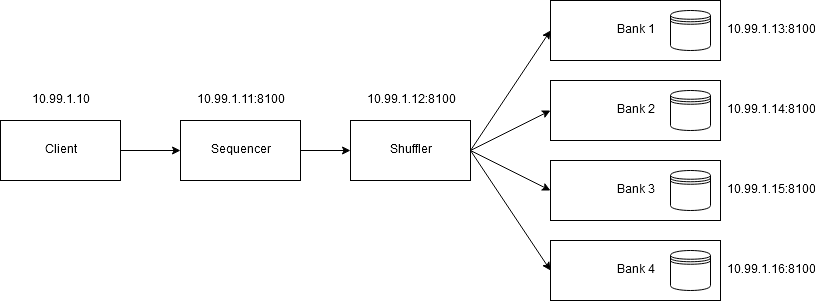
\includegraphics[width=15cm]{topology.png}
		\caption{Topologie systému}
		\label{fig:topology.pdf_tex}
	\end{figure}
	
	\subsection{Obecná struktura projektu}
	Zdrojové kódy projektu se nachází ve složce \verb|src|. Každý server je umístěn ve vlastní složce (\verb|client|, \verb|bank-1|, ...). V adresáři \verb|src| je také umístěn \verb|Vagrantfile| obsahující konfiguraci nasazení virtuálních strojů. 
	
	Server je tvořen python skriptem, konfiguračním souborem pro \verb|upstart| a skriptem \verb|bootstrap.sh|, který server inicializuje a spouští. Každý server je na virtuálním stroji veden jako služba. Tím je možné daný server pohodlně vypínat/zapínat. 	Každý ze serverů loguje svou činnost do souboru \verb|log.txt|, skrze který je možné za běhu kontrolovat stav systému. 
	
	\begin{figure}[H]
		\centering
		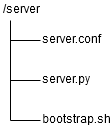
\includegraphics[width=2.5cm]{server-structure.png}
		\caption{Obecná struktura složky serveru}
		\label{fig:serv-struct.pdf_tex}
	\end{figure}
	
	\subsection{Client}
	Klient je ze všech modulů nejjednodušší, neobsahuje vlastní server a pouze generuje pokyny k transakcím. Počet pokynu, který má klient generovat a adresa sekvenceru jsou skriptu předány parametrem při spuštění.
	
	\subsection{Shuffler}
	Shuffler má interní frontu (o velikosti 10) do které ukládá pokyny k operacím přijaté od sekvenceru. Po naplnění je fronta zpřeházena a pokyny jsou postupně odeslány na všechny bankovní servery.
	
	Adresy bankovních serverů jsou načítány z konfiguračního JSON souboru, jehož cesta je shuffleru předána parametrem.
	
	\subsection{Bank N}
	Bankovní server přijímá pokyny k transakcím od shuffleru a ukládá je do interní haldy. Na vrchu této haldy je pokyn s nejmenším časovým razítkem (ta generuje sekvencer). Při spuštění bankovního serveru je nastaven interní čítač očekávaných id na hodnotu, která musí odpovídat prvnímu id generovanému sekvencerem. Pokud je na vrcholu haldy pokyn s $id = expected\_id$, je vyjmut a proveden. 	Po každé provedené transakci je do souboru \verb|balance.txt| zapsán současný zůstatek na účtě. 
	
	Vzhledem k nutnosti 'synchronizace' prvního id generovaného sekvencerem a počátečního \verb|expected_id| bankovního serveru je v případě restartu sekvenceru nutné restartovat také všechny bankovní servery (a naopak).
	
	Každý bankovní server má vlastní databázi běžící na daném virtuálním stroji.

	
	\section{Spuštění}
	
	Systém je možné spustit příkazem \verb|vagrant up| v adresáři \verb|src|. Stav klienta je možné kontrolovat skrze ssh na vrituální stroj příkazem \verb|status client|. V případě, že klient doběhl, jeho status bude \verb|stop/waiting|.
	
	Po doběhnutí klienta lze zkontrolovat zůstatky bankovních serverů. Zůstatek je na každém serveru uložen v souboru \verb|/home/vagrant/bank/balance.txt|.
	
	\section{Závěr}
	Práci se mi podařilo úspěšně implementovat. Míchání požadavků shufflerem by bylo lepší realizovat skrze náhodné zpoždění, systém by tak více odrážel reálný stav. Zapisovat aktuální zůstatek na účte do souboru po každé provedené transakci je není obecně dobrá praktika, ale zde to usnadňuje testování a kontrolu výsledků.
	
\end{document}
